\documentclass[12pt]{article}
\usepackage{graphicx}
\usepackage{float}
\usepackage[margin=1in]{geometry}
\title{Null Distributions and Coverage}
\date{}
\begin{document}
%\maketitle
\begin{center}\section*{Null Distributions and Coverage}\end{center}
\section{Simulated Data}
\subsection*{2x Noise}
\begin{figure}[H]
\centerline{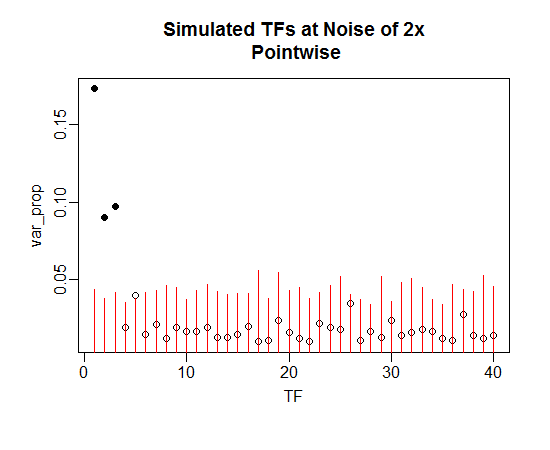
\includegraphics[scale=.5]{noise2p}}
\caption{\it Variable Inclusion Frequencies with point-wise 95\% null bands.}\label{fig:f1}  
\end{figure}


\begin{figure}[H]
\centerline{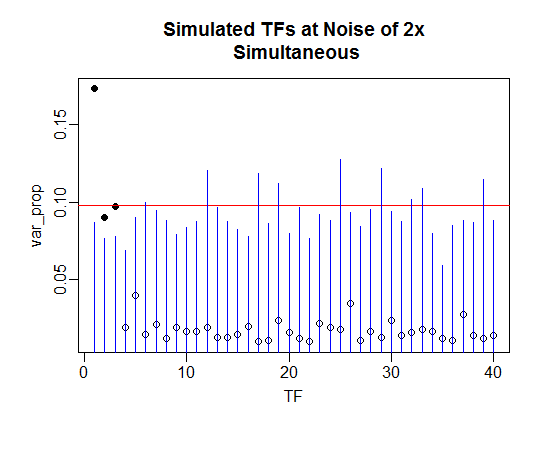
\includegraphics[scale=.5]{noise2s}}
\caption{\it Variable Inclusion Frequencies with simultaneous 95\% null bands (blue) and $95^{th}$ quantile of maximum cut-off (red).}
\end{figure}


\subsection*{5x Noise}
\begin{figure}[H]
\centerline{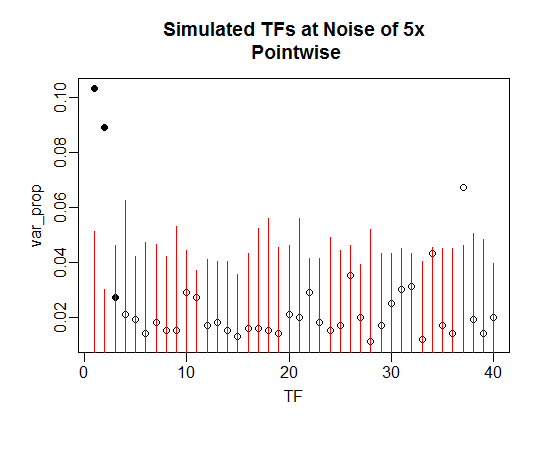
\includegraphics[scale=.5]{noise5p}}
\caption{\it Variable Inclusion Frequencies with point-wise 95\% null bands.}\label{fig:f1}  
\end{figure}


\begin{figure}[H]
\centerline{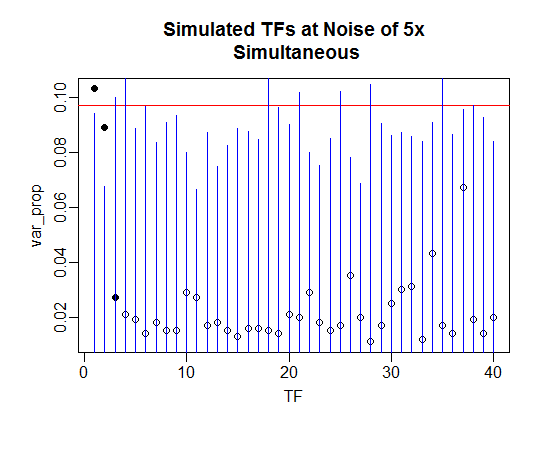
\includegraphics[scale=.5]{noise5s}}
\caption{\it Variable Inclusion Frequencies with simultaneous 95\% null bands (blue) and $95^{th}$ quantile of maximum cut-off (red).}\label{fig:f1}  
\end{figure}
\newpage
\section{Actual Data}
\begin{figure}[H]
\centerline{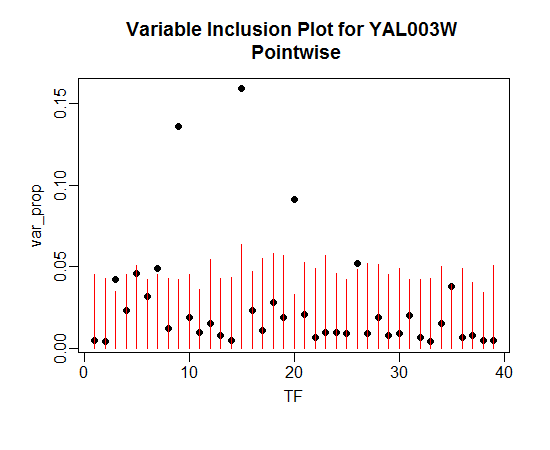
\includegraphics[scale=.5]{gene3p}}
\caption{\it Variable Inclusion Frequencies with point-wise 95\% null bands.}\label{fig:f1}  
\end{figure}


\begin{figure}[H]
\centerline{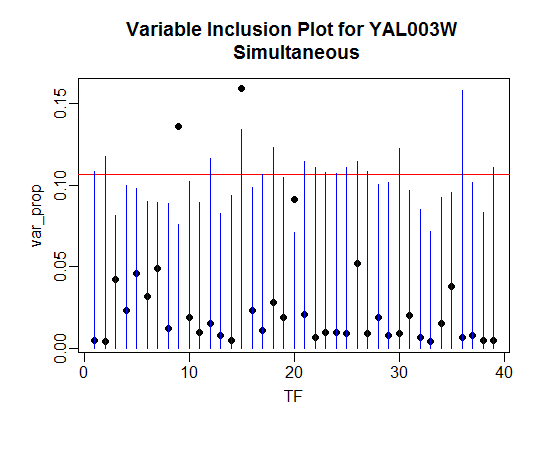
\includegraphics[scale=.5]{gene3s}}
\caption{\it Variable Inclusion Frequencies with simultaneous 95\% null bands (blue) and $95^{th}$ quantile of maximum cut-off (red).}\label{fig:f1}  
\end{figure}
\begin{figure}[H]
\centerline{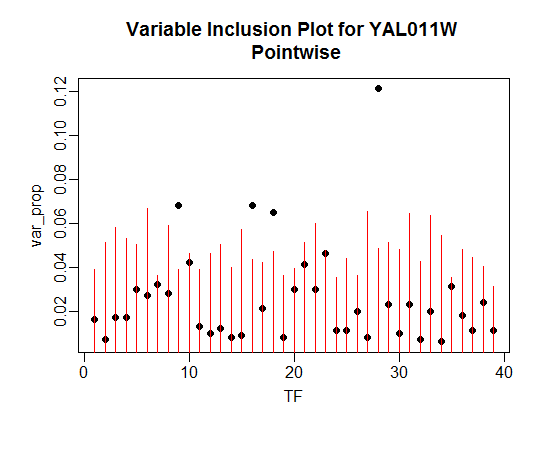
\includegraphics[scale=.5]{gene10p}}
\caption{\it Variable Inclusion Frequencies with point-wise 95\% null bands.}\label{fig:f1}  
\end{figure}


\begin{figure}[H]
\centerline{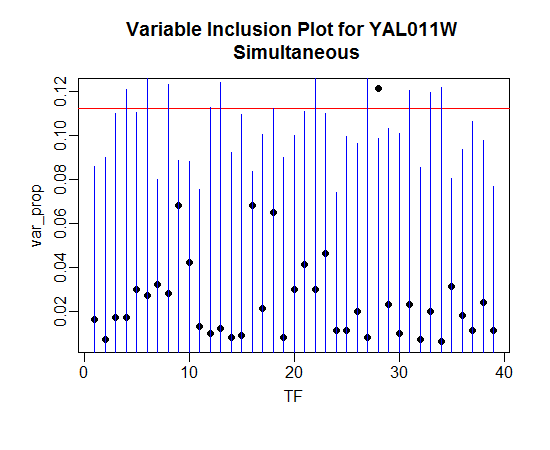
\includegraphics[scale=.5]{gene10s}}
\caption{\it Variable Inclusion Frequencies with simultaneous 95\% null bands (blue) and $95^{th}$ quantile of maximum cut-off (red).}\label{fig:f1}  
\end{figure}
\end{document}